%%=============================================================================
%% Gebruikte technologieën
%%=============================================================================

\chapter{Gebruikte technologieën}
\label{ch:technologie}

%% TODO: Hoe ben je te werk gegaan? Verdeel je onderzoek in grote fasen, en
%% licht in elke fase toe welke stappen je gevolgd hebt. Verantwoord waarom je
%% op deze manier te werk gegaan bent. Je moet kunnen aantonen dat je de best
%% mogelijke manier toegepast hebt om een antwoord te vinden op de
%% onderzoeksvraag.


\section{Spring en Spring Boot}
\label{sec:spring-boot}

Dit onderzoek maakt gebruik van Spring Boot om microservices op te stellen. Hieronder volgt een inleiding tot het Spring framework en het verschil tussen Spring en Spring Boot.

Het Spring framework is een open source framework gericht op applicatieontwikkeling in Java~\autocite{Spring2014}. Het bekendste onderdeel van het framework is het Inversion of Control (IoC) principe, ook gekend als dependency injection. Dit betekent onder andere dat een object geannoteerd kan worden met \texttt{@Component} en Spring zal het object aanmaken, alle nodige velden vullen en het object toevoegen aan de context van de applicatie. Op deze manier is het mogelijk om verschillende objecten toe te voegen aan de context, zodat ze onderling gemakkelijk samenwerken. Het IoC principe vergemakklijkt hierdoor de manier om andere bibliotheken te integreren in de applicatie.

Spring Boot kan gezien worden als een uitbreiding op het Spring framework. Het maakt het gemakkelijk om op zichzelf staande, productiewaardige Spring applicaties te maken waar het niet nodig is om veel aan de configuratie te sleutelen~\autocite{SpringBoot2015}. Het mantra van Spring Boot is dan ook \textit{convention-over-configuration}. Dit is bijzonder handig voor microservices omdat bijvoorbeeld een eenvoudige REST applicatie aangemaakt kan worden in minder dan 20 lijnen code.

\begin{lstlisting}[language=Java, basicstyle=\ttfamily\small, caption=eenvoudige Spring Boot REST app]
@Controller
@EnableAutoConfiguration
public class SampleController {

    @RequestMapping("/")
    @ResponseBody
    String home() {
        return "Hello World!";
    }

    public static void main(String[] args) throws Exception {
        SpringApplication.run(SampleController.class, args);
    }
}
\end{lstlisting}

De \texttt{@Controller} annotatie zorgt ervoor dat de klasse gebruikt kan worden door Spring MVC om web requests te behandelen. \texttt{@RestController} kan vanaf Spring 4.0 gebruikt worden, deze combineert de annotaties \texttt{@Controller} en \texttt{@ResponseBody}. De laatste annotatie is handig om \texttt{return} waarden van requests op te vangen in een zelfgedefinieerde Java klasse. \texttt{@EnableAutoConfiguration} zegt dat Spring Boot de applicatie automatisch moet configureren op basis van de toegevoegde bibliotheken. Ten slotte is er nog de \texttt{@RequestMapping} annotatie die Spring vertelt dat het pad \texttt{/} gemapped moet worden op de \texttt{home} methode.

Omdat met Spring Boot zo weinig mogelijk aan de configuratie gesleuteld dient te worden, werd dit framework gekozen als platform voor de microservices in dit onderzoek.

\section{Containerisatie met Docker}
\label{sec:docker}

Docker is een open-source platform met als doel het opzetten van applicaties te automatiseren~\autocite{Docker2016}. Elke microservice, bijvoorbeeld een Spring Boot applicatie, kan door Docker uitgevoerd worden in zijn eigen container. De verschillende containers zijn geïsoleerd van elkaar en delen enkel de minimale kernel van het besturingssysteem. Containers lijken op het eerste zicht op virtuele machines, in het opzicht dat beide geïsoleerde omgevingen zijn die beheerd worden door een controlerend proces: een container manager en hypervisor respectievelijk. Het grootste verschil tussen de twee is echter dat, voor elke virtuele machine, een volledige stack van componenten uitgevoerd dienen te worden: het besturingssysteem tot en met de applicatielaag en de virtuele hardware met netwerkkaarten, CPU's en geheugen (zie figuur \ref{fig:vm_stack}).

\begin{figure}
\caption{Virtuele machine stack}
\centering
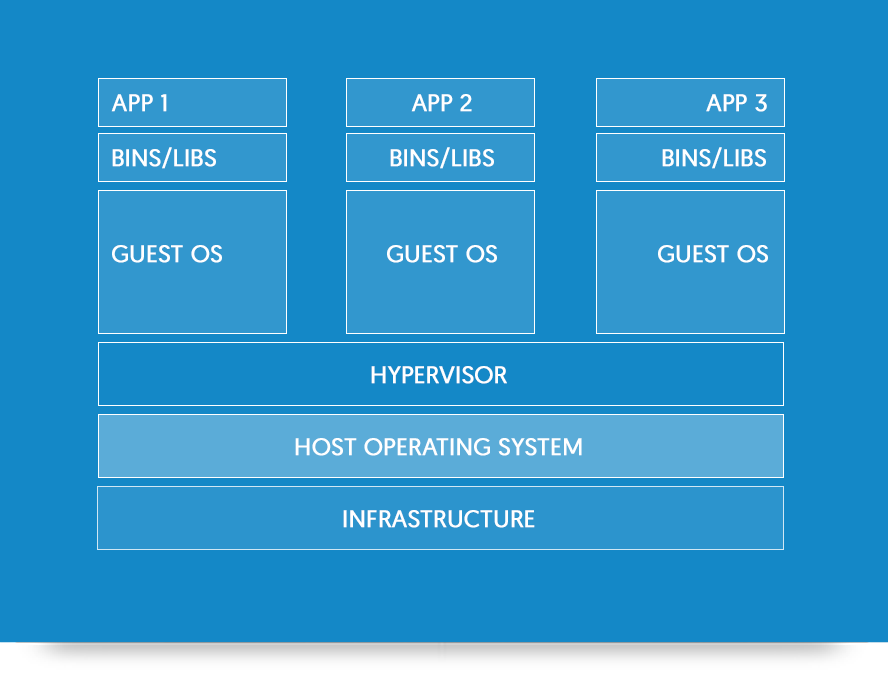
\includegraphics[width=1\textwidth]{docker_VMs}
\label{fig:vm_stack}
\end{figure}

\begin{figure}
\caption{Docker container stack}
\centering
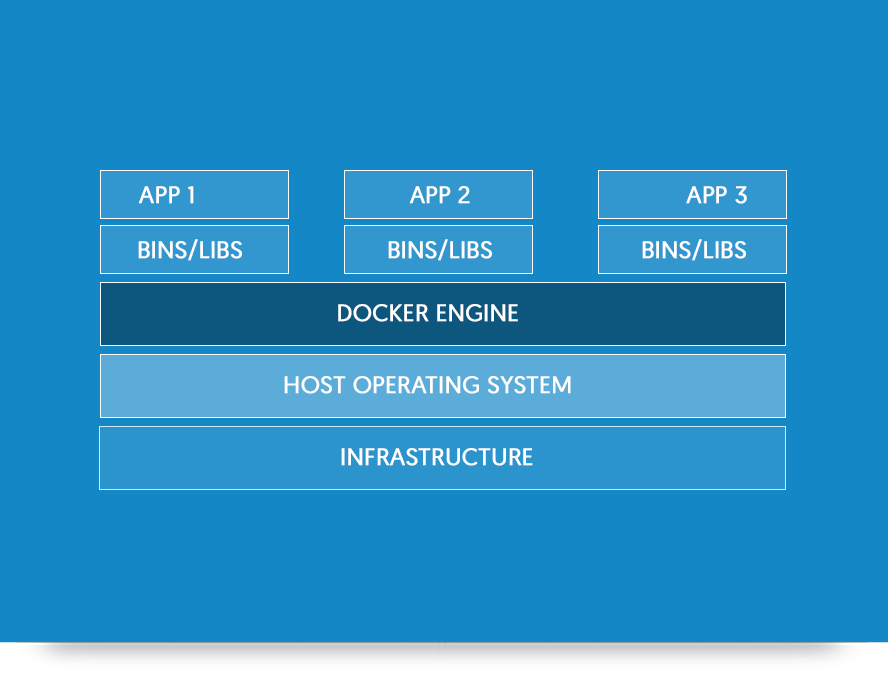
\includegraphics[width=1\textwidth]{docker_containers}
\label{fig:container_stack}
\end{figure}

Containers daarentegen functioneren eerder als volledig geïsoleerde \textit{sandboxes}. De containers delen met elkaar de kernel van het besturingssysteem met de aanwezige systeembronnen (zie figuur \ref{fig:container_stack}). Dit betekent dat containers veel minder zwaar zijn op het onderliggende systeem, zodat meer containers uitgevoerd kunnen worden dan virtuele machines. Een belangrijke limitatie van containers is echter dat ze enkel uitgevoerd kunnen worden in Linux-gebaseerde besturingssystemen. Dit omdat Docker gebruik maakt van kernel isolatie, wat een specifieke Linux technologie is.

Docker kan niet rechtstreeks uitgevoerd worden op Mac of Windows systemen, maar er is een eenvoudige workaround om dit te verhelpen: Docker Toolbox. Er zal eerst een Linux virtuele machine opgestart worden in VirtualBox, waarna de docker containers uitgevoerd kunnen worden in deze virtuele machine.

\section{Tracing}
\label{sec:tracing}

Een van de uitdagingen in een microservice omgeving is om het overzicht te bewaren hoe alle verschillende services met elkaar samenwerken. Omdat elke service onafhankelijk is van de volgende, is het moeilijker om het gedrag van het volledige systeem te controleren. Zoals eerder vermeld in \ref{ch:inleiding} kan tracing hierbij helpen en omdat het gaat over tracing in een microservice systeem, spreekt men ook over distributed tracing.

\subsection{Spring Cloud Sleuth}
\label{sec:sleuth}

Spring Cloud biedt een aantal bibliotheken aan zoals Config (een plaats om configuraties van verschillende microservices te beheren), Netflix (Netflix OSS integraties voor Spring Boot apps zoals Eureka) en dus ook Sleuth~\autocite{SpringCloud2015}. Sleuth is een distributed tracing oplossing die concepten van Dapper, Zipkin en HTrace leent.

Een trace ziet er bij Sleuth uit zoals bij Dapper. Het bevat een trace id dat gevormd wordt wanneer de eerste request gemaakt wordt. Voor elke service die de request doorkruist, wordt een span id toegekend voor die service en toegevoegd aan de trace. Zie figuur \ref{fig:dapper_trace} als voorbeeld. Op de afbeelding hebben alle 5 spans dezelfde trace id (niet getoond op de figuur). Bij Sleuth is het zo dat de eerste span van een trace dezelfde id kent voor zowel span en trace id. Sleuth zal er dan voor zorgen dat die id's, samen met responstijd data, toegevoegd worden aan de headers in de request responses.

\begin{figure}
\caption{Voorbeeld van een trace met 5 spans}
\centering
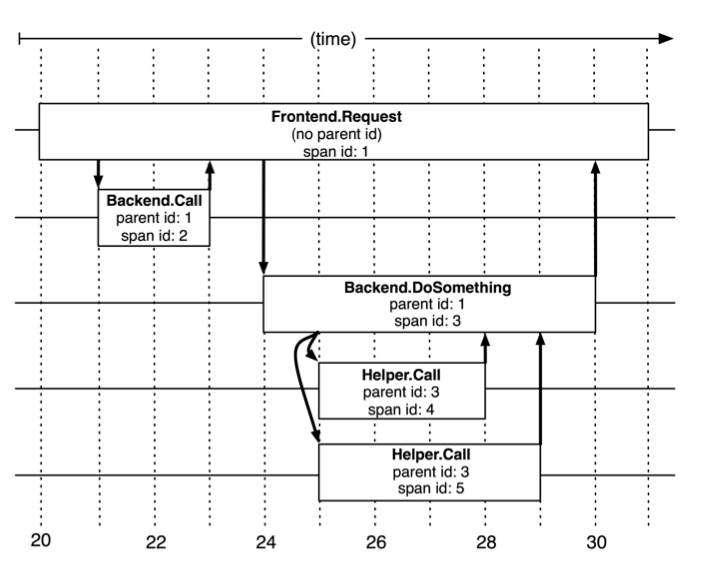
\includegraphics[width=1\textwidth]{dapper_trace}
\label{fig:dapper_trace}
\end{figure}

Sleuth voegt de trace en span id's ook toe aan de logging voor de microservice. Dit ziet er zo uit: \texttt{[my-service-id,73b62c0f90d11e06,73b62c0f90d11e06,false]}. \texttt{my-service-id} is de naam van de service, de eerste id duidt de trace aan, de volgende is de span en de laatste waarde geeft aan of de span geëxporteerd dient te worden naar Zipkin.

\subsection{Zipkin}
\label{sec:zipkin}

Zipkin is een open source project dat helpt bij het verzamelen en visualiseren van tracing data om responstijd problemen in microservice architecturen te kunnen detecteren~\autocite{Zipkin2016}.

Sleuth heeft de mogelijkheid om tracing informatie te sturen naar een Zipkin server door de dependency \texttt{spring-cloud-sleuth-zipkin} toe te voegen aan de applicatie. Sleuth gaat er standaard vanuit dat de Zipkin server loopt op \texttt{http://localhost:9411}. De locatie kan echter aangepast worden door \texttt{spring.zipkin.baseUrl} toe te voegen aan de applicatie eigenschappen (application.properties).

\section{Logging}
\label{sec:logging}

Als er iets vreemd wordt opgemerkt in de tracing informatie die Zipkin visualiseert, kan er worden afgeleid in welke service het probleem zich situeert, maar niet wat dat probleem altijd is. Om problemen op te lossen, dient de beheerder van de microservices zich te verdiepen in log bestanden. Als hulpmiddel hiervoor kan de ELK stack van pas komen. ELK staat voor ElasticSearch, Logstash en Kibana. Logstash verzamelt de logs van een microservice en stuurt deze naar een ElasticSearch server die de logs indexeert. De Kibana server is de UI die de logs uit ElasticSearch leest en ze op een gebruiksvriendelijke manier weergeeft. Met Kibana is het dan mogelijk om bijvoorbeeld alle logs van een bepaalde trace weer te geven door te filteren op trace id. Als log shipper kan ook Fluentd gebruikt worden in plaats van Logstash. In dit onderzoek wordt bekeken welke log shipper het meest performant is